\documentclass[11pt]{article}




\usepackage{color}
\usepackage{verbatim}
\usepackage{amsmath}
\usepackage{amsfonts}
\usepackage{url}

\newcommand{\notes}[1]{\textcolor{red}{#1}}
\newcommand{\adjmat}{\mathbf{Y}}
\newcommand{\obsadj}{\mathbf{y}}
\newcommand{\grphSpace}{\mathcal{Y}}
\newcommand{\dyadSpace}{\mathbb{Y}}
\newcommand{\form}{^+}
\newcommand{\diss}{^-}
\newcommand{\paramVec}{\theta}
\newcommand{\covmat}{\mathbf{X}}




\usepackage{Sweave}
\begin{document}

\title{NIMD 2012 - STERGM labs}
\maketitle

\tableofcontents


\section{Notes on model specification and syntax}
Within \emph{statnet}, an ERGM involves one network and one set of network statistics, so these are specified together using R's formula notation:

\begin{center}
\texttt{my.network $\sim$ my.vector.of.g.statistics}
\end{center}

For a call to \texttt{stergm}, there is still one network, but two formulas. These are now passed as three separate arguments: the network (argument \texttt{nw}), the formation formula (argument \texttt{formation}), 
and the dissolution formula (argument \texttt{dissolution}).  The latter two both take the form of a one-sided formula.  E.g.:

\begin{verbatim}
        stergm(my.network,
            formation= ~edges+kstar(2),
            dissolution= ~edges+triangle
        )
\end{verbatim}

There are other features of a call to either \texttt{ergm} or \texttt{stergm} that will be important for us here. 
We list the features here; each is illustrated in one or more examples below.

\begin{enumerate}

\item{To fix the coefficient for a particular network statistic, one uses offset notation.  
For instance, to fix a dissolution model with only an edges term with parameter value 4.2, the dissolution formula woud be:

\begin{center}
\texttt{dissolution= $\sim$offset(edges)}
\end{center}

and the corresponding argument for passing the parameter value would be:

\begin{center}
\texttt{offset.coef.diss = 4.2}
\end{center}

}

\item{In parallel with \texttt{ergm}, any information used to specify the nature of the fitting algorithm is passed by specifying a vector called \texttt{control.stergm} 
to the \texttt{control} argument. For example:
	
\begin{center}
\texttt{control=control.stergm(MCMC.burnin=10000)}
\end{center}

For a list of options, type \texttt{?control.stergm}
}
  
\item{Another argument that the user must supply is \texttt{estimate}, which controls the estimation method. 
Unlike with cross-sectional ERGMs, there is not necessarily an obvious default here, as different scenarios are best fit with different approaches.
The most important for the new user to recognize are \texttt{EGMME} (equilibrium generalized method of moments estimation) and \texttt{CMLE} (conditional maximum likelihood estimation). 
A good rule of thumb is that when fitting to two networks, one should use \texttt{estimate="CMLE"} while when fitting to a single cross-section with some duration information, 
use \texttt{estimate="EGMME"}.
}

\item{For cross-sectional ERGMs, the model is by default fit using the sufficient statistics present in the cross-sectional network.  
For STERGMs, the presence of multiple models makes the default less clear.  Thus, the user is required to supply this information via the \texttt{targets} argument.  
This can take a one-sided formula listing the terms to be fit; or, if the formula is identical to either the formation or dissolution model, 
the user can simply pass the string \texttt{"formation"} or \texttt{"dissolution"}, respectively. If one is specifying
targets=``formation'', dissolution should be an offset, and vice versa.
If the values to be targeted for those terms are anything other than the sufficient statistics present in the cross-sectional network, 
then those values can be passed with the argument \texttt{target.stats}.

}

\end{enumerate}


\section{Example 1: Estimation with two network cross-sections}

We begin with an example whose structure and syntax bears the most resemblance to the ERGMs that we are used to. 
This is the case where we have two observations of network structure at two or more points in time on the same node set.  
Many classic network studies were of this type, and data of this form continue to be collected and analyzed in many fields.

Let us consider the first two time points in the famous Sampson monastery data:

\begin{Schunk}
\begin{Sinput}
> data(samplk)
> ls(pattern="samp*")
\end{Sinput}
\begin{Soutput}
[1] "samp"            "samp.stergm.fit" "samplk1"        
[4] "samplk2"         "samplk3"        
\end{Soutput}
\end{Schunk}

To pass them into \texttt{stergm}, we need to combine them into a list:
\begin{Schunk}
\begin{Sinput}
> samp <- list()
> samp[[1]] <- samplk1
> samp[[2]] <- samplk2
> 
\end{Sinput}
\end{Schunk}

Now we must decide on a model to fit to them.  Plotting one network:

\begin{center}
\begin{Schunk}
\begin{Sinput}
> plot(samplk1)
\end{Sinput}
\end{Schunk}
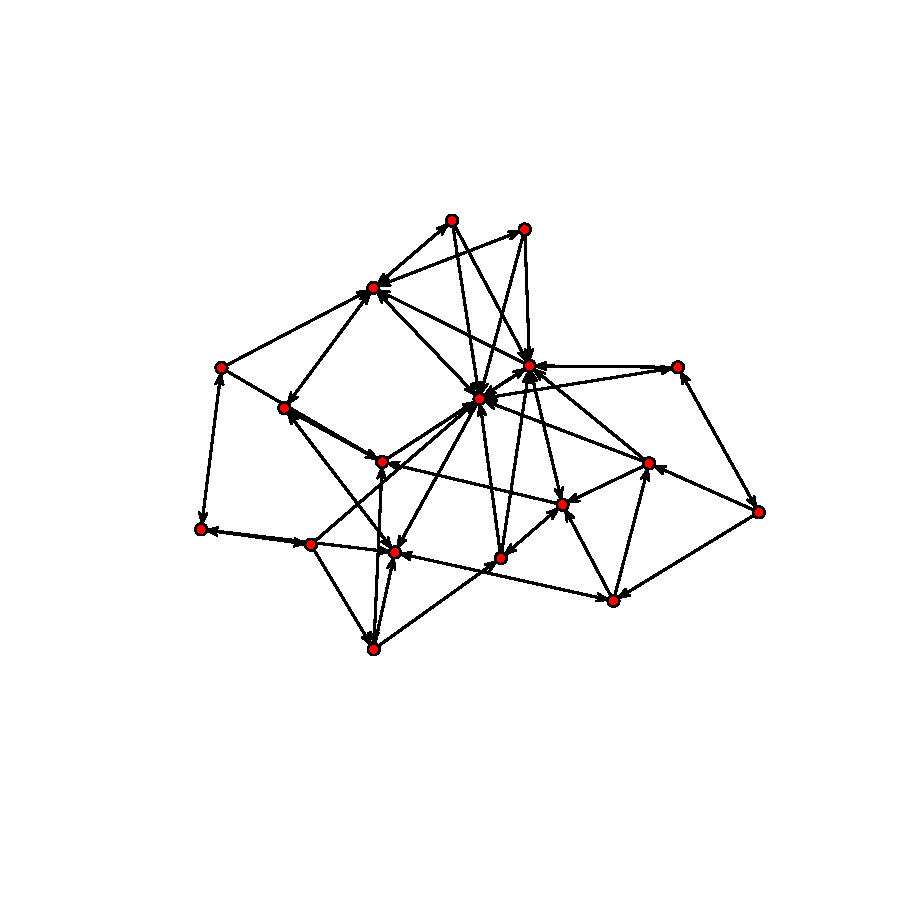
\includegraphics{STERGM-005}
\end{center}



\noindent we might get the idea to consider mutuality as a predictor of a directed edge.  Also, since this is a directed network, 
and there appear to be a considerable number of triadic relations, it might be worth investigating the role of cyclic vs. transitive triads in the network.
Of course, since we have two network snapshots, and we have separate formation and dissolution models, 
we can estimate the degree to which closing a mutual dyad or closing a triad of each type predicts the creation of a tie, 
and also estimate the degree to which maintaining a mutual dyad or maintaining a triad of each type predicts the persistence of an existing tie. 
We might see different phenomena at work in each case; or the same phenomena, but with different coefficients.


\begin{Schunk}
\begin{Sinput}
> samp.stergm.fit <- stergm(samp,
 	formation= ~edges+mutual+ctriad+ttriad,
 	dissolution = ~edges+mutual+ctriad+ttriad,
 	estimate = "CMLE"
 	)
\end{Sinput}
\end{Schunk}

\texttt{Fitting formation:}\\
\texttt{Iteration 1 of at most 20:}\\
$\Rightarrow$ Lots of output snipped. $\Leftarrow$\\
\texttt{Time points not specified for a list. Modeling transition from the first to the second network. This behavior may change in the future.}\\



And the results:



\begin{Schunk}
\begin{Sinput}
> summary(samp.stergm.fit)
\end{Sinput}
\begin{Soutput}
==============================
Summary of formation model fit 
==============================

Formula:   ~edges + mutual + ctriad + ttriad

Iterations:  20 

Monte Carlo MLE Results:
        Estimate Std. Error MCMC % p-value    
edges    -3.5554     0.4643      4 < 1e-04 ***
mutual    2.2509     0.5895      1 0.00017 ***
ctriple  -0.4956     0.3676      0 0.17880    
ttriple   0.2929     0.1288      2 0.02385 *  
---
Signif. codes:  0 �***� 0.001 �**� 0.01 �*� 0.05 �.� 0.1 � � 1 

     Null Deviance:    0  on 251  degrees of freedom
 Residual Deviance: -219  on 247  degrees of freedom
 
AIC: -211    BIC: -196.9    (Smaller is better.) 

================================
Summary of dissolution model fit
================================

Formula:   ~edges + mutual + ctriad + ttriad

Iterations:  20 

Monte Carlo MLE Results:
        Estimate Std. Error MCMC % p-value  
edges    -0.1253     0.4293      0  0.7716  
mutual    1.5773     0.7841      0  0.0496 *
ctriple  -1.7017     1.2156      0  0.1676  
ttriple   0.6931     0.3724      0  0.0685 .
---
Signif. codes:  0 �***� 0.001 �**� 0.01 �*� 0.05 �.� 0.1 � � 1 

     Null Deviance:   0.00  on 55  degrees of freedom
 Residual Deviance: -10.51  on 51  degrees of freedom
 
AIC: -2.507    BIC: 5.522    (Smaller is better.) 
\end{Soutput}
\begin{Sinput}
> 
\end{Sinput}
\end{Schunk}



So, a relationship is more likely than chance to form if it will close a mutual pair. 
And it is also more likely than chance to persist if it will retain a mutual pair, although the coefficient is smaller.
A relationship is more likely than chance to form if it will close a transitive triad, and more likely to persist if it 
sustains a transitive triad, although these effects appear to be less clearly significant. 



\section{Example 2: Estimation and simulation with a cross-sectional network and durational information}

Let us imagine that we have observed two things: a cross-sectional network, and a mean relational duration. 
For the network, we will use Padgett's well-known ``flobusiness'' data set.  And we will assume that we have somehow measured a mean relational duration of 10 time steps. 
Furthermore, we are willing to (for reasons of theory or convenience) assume a purely homogeneous dissolution process 
(that is, every existing relationship has the same probability of dissolving as all others, and at all times).  
For a cross-sectional ERGM, a purely homogeneous model is one with just a single term in it for an edge count. 
The same is true for either of the two formulas in a STERGM.  

First, take a lok at the data:
\begin{Schunk}
\begin{Sinput}
> data(florentine)
> ls()
\end{Sinput}
\begin{Soutput}
[1] "flo.stergm.fit"  "flobusiness"     "flomarriage"    
[4] "samp"            "samp.stergm.fit" "samplk1"        
[7] "samplk2"         "samplk3"         "theta.diss"     
\end{Soutput}
\begin{Sinput}
> flobusiness
\end{Sinput}
\begin{Soutput}
 Network attributes:
  vertices = 16 
  directed = FALSE 
  hyper = FALSE 
  loops = FALSE 
  multiple = FALSE 
  bipartite = FALSE 
  total edges= 15 
    missing edges= 0 
    non-missing edges= 15 

 Vertex attribute names: 
    priorates totalties vertex.names wealth 
\end{Soutput}
\end{Schunk}

\begin{center}
\begin{Schunk}
\begin{Sinput}
> plot(flobusiness)
\end{Sinput}
\end{Schunk}
\includegraphics{STERGM-009}
\end{center}

The steps we will go through are:

\begin{enumerate}

\item Specify formation and dissolution models (\texttt{formation} and \texttt{dissolution}).

We will begin by assuming a formation model.  From looking at the visualization of the data, it certianly appears as if some triangle-level clustering is occurring. 
We can aim to capture that by using a \texttt{gwesp} term.

\begin{center}
\texttt{formation = $\sim$edges+gwesp(0,fixed=T)}
\end{center}

Analogously to cross-sectional ERGMs, our assumption of completely homogeneous dissolution corresponds to a model with only an edgecount term in it.  In STERGM notation this is:

\begin{center}
\texttt{dissolution = $\sim$edges}
\end{center}

\item Calculate \texttt{theta.diss}.

Because this is a discrete memoryless process, we have the relationship:
\begin{equation}
\theta = \ln{(d-1)}
\end{equation}
So, for our dissolution model, theta.diss = $\ln{(10-1)}$ = $\ln{9}$ = $2.197$:

\begin{Schunk}
\begin{Sinput}
> theta.diss <- log(9)
\end{Sinput}
\end{Schunk}

In short, because our dissolution model is dyadic independent, we can calculate it using a (rather simple) closed form solution.

\item Estimate the formation model, conditional on the dissolution model.
We put it all together for our first call to \texttt{stergm}, adding in one additional control argument that helps immensely with monitoring model convergence (and is just plain cool): 
plotting the progress of the coefficient estimates and the simulated sufficient statistics in real time.

\begin{Schunk}
\begin{Sinput}
> flo.stergm.fit <- stergm(flobusiness,
 	formation= ~edges+gwesp(0,fixed=T),
 	dissolution = ~offset(edges),
 	targets="formation",
 	offset.coef.diss = theta.diss,
 	estimate = "EGMME",
 	control=control.stergm(SA.plot.progress=TRUE)
 )
\end{Sinput}
\end{Schunk}
\texttt{Iteration 1 of at most 20:}\\
$\Rightarrow$ Lots of output snipped. $\Leftarrow$ \\
\texttt{== Phase 3: Simulate from the fit and estimate standard errors.==}

First, we should double-check to make sure the fitting went well:
\begin{Schunk}
\begin{Sinput}
> mcmc.diagnostics(flo.stergm.fit)
\end{Sinput}
\end{Schunk}

\begin{verbatim}
==========================
EGMME diagnostics
==========================
\end{verbatim}

$\Rightarrow$ Lots of output snipped. $\Leftarrow$\\

\begin{figure}[h]
\begin{center}
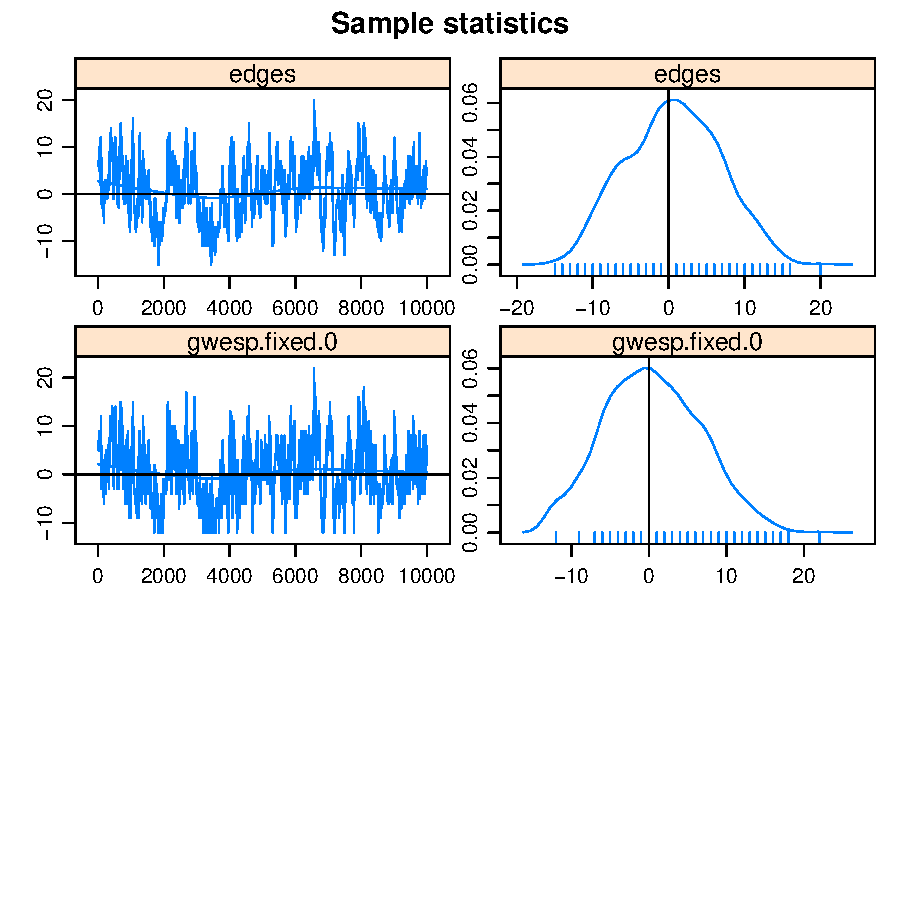
\includegraphics[height=3in]{STERGM-fit1diag}
\end{center}
\end{figure}

Since those look good, we can next query the object in a variety of ways to see what we have:
\begin{Schunk}
\begin{Sinput}
> flo.stergm.fit
\end{Sinput}
\begin{Soutput}
Formation Coefficients:
        edges  gwesp.fixed.0  
       -6.491          2.344  
Dissolution Coefficients:
edges  
2.197  
\end{Soutput}
\begin{Sinput}
> names(flo.stergm.fit)
\end{Sinput}
\begin{Soutput}
 [1] "network"         "formation"       "dissolution"    
 [4] "targets"         "target.stats"    "estimate"       
 [7] "covar"           "opt.history"     "sample"         
[10] "sample.obs"      "control"         "reference"      
[13] "formation.fit"   "dissolution.fit"
\end{Soutput}
\begin{Sinput}
> flo.stergm.fit$formation
\end{Sinput}
\begin{Soutput}
~edges + gwesp(0, fixed = T)
\end{Soutput}
\begin{Sinput}
> flo.stergm.fit$formation.fit
\end{Sinput}
\begin{Soutput}
MLE Coefficients:
        edges  gwesp.fixed.0  
       -6.491          2.344  
\end{Soutput}
\begin{Sinput}
> summary(flo.stergm.fit)
\end{Sinput}
\begin{Soutput}
==============================
Summary of formation model fit 
==============================

Formula:   ~edges + gwesp(0, fixed = T)

Iterations:  NA 

Equilibrium Generalized Method of Moments Results:
              Estimate Std. Error MCMC %  p-value    
edges          -6.4913     0.5342     NA  < 1e-04 ***
gwesp.fixed.0   2.3440     0.6067     NA 0.000183 ***
---
Signif. codes:  0 �***� 0.001 �**� 0.01 �*� 0.05 �.� 0.1 � � 1 

Warning:  The standard errors do not incorporate uncertainty due to the "noisy" estimation procedure.


================================
Summary of dissolution model fit
================================

Formula:   ~offset(edges)

Iterations:  NA 

Equilibrium Generalized Method of Moments Results:
      Estimate Std. Error MCMC % p-value
edges    2.197         NA     NA      NA

Warning:  The standard errors do not incorporate uncertainty due to the "noisy" estimation procedure.


 The following terms are fixed by offset and are not estimated:
  edges 
\end{Soutput}
\end{Schunk}
\end{enumerate}

We have now obtained estimates for the coefficients of a formation model that, 
conditional on the stated dissolution model, yields simulated targets that matched those observed.
Something very useful we have also gained in the process is the ability to simulate networks with the 
desired cross-sectional structure and mean relational duration.  This ability serves us well for any application 
areas that requires us to simulate phenomena on dynamic networks, whether they entail the diffusion of information or disease, or some other process.  

\begin{Schunk}
\begin{Sinput}
> flo.stergm.sim <- simulate.stergm(flo.stergm.fit, nsim=1, 
     time.slices = 1000)
\end{Sinput}
\end{Schunk}

In order to undestand the results, we must have a brief tutorial in objects of class \texttt{networkDynamic} and the \emph{networkDynamic} package.

\section{networkDynamic}

In \emph{statnet}, cross-sectional networks are stored using objects of class \emph{network}.  
Tools to create, edit, and query network objects are in the package \emph{network}. Dynamic networks 
are now stored as objects with two classes (\emph{network} and \emph{networkDynamic}).
They can thus be edited or queried using standard functions from the \emph{network} package, or using additional 
functions tailored specifically to the case of dynamic networks in the package \emph{networkDynamic}.

To illustrate, let us begin with the network that we just created:

\begin{Schunk}
\begin{Sinput}
> flo.stergm.sim
\end{Sinput}
\begin{Soutput}
 Network attributes:
  vertices = 16 
  directed = FALSE 
  hyper = FALSE 
  loops = FALSE 
  multiple = FALSE 
  bipartite = FALSE 
  total edges= 120 
    missing edges= 0 
    non-missing edges= 120 

 Vertex attribute names: 
    priorates totalties vertex.names wealth 
\end{Soutput}
\end{Schunk}

We can deduce from the number of edges that this likely represents the cumulative network---that is, the union of all edges that exist at any point in time over the course of the simulation.  
What does the network look like at different time points? The function \texttt{network.extract} allows us to pull out the network at an instantanoues time point (with the argument \texttt{at}),
or over any given spell (with the arguments \texttt{onset} and \texttt{terminus}).

\begin{Schunk}
\begin{Sinput}
> net <- network.extract(flo.stergm.sim,at=429)
> net
\end{Sinput}
\begin{Soutput}
 Network attributes:
  vertices = 16 
  directed = FALSE 
  hyper = FALSE 
  loops = FALSE 
  multiple = FALSE 
  bipartite = FALSE 
  total edges= 23 
    missing edges= 0 
    non-missing edges= 23 

 Vertex attribute names: 
    priorates totalties vertex.names wealth 
\end{Soutput}
\end{Schunk}

For any one of these time points, we can look at the network structure:

\begin{Schunk}
\begin{Sinput}
> plot(network.extract(flo.stergm.sim,at=882))
\end{Sinput}
\end{Schunk}

\begin{figure}[ht]
\begin{center}
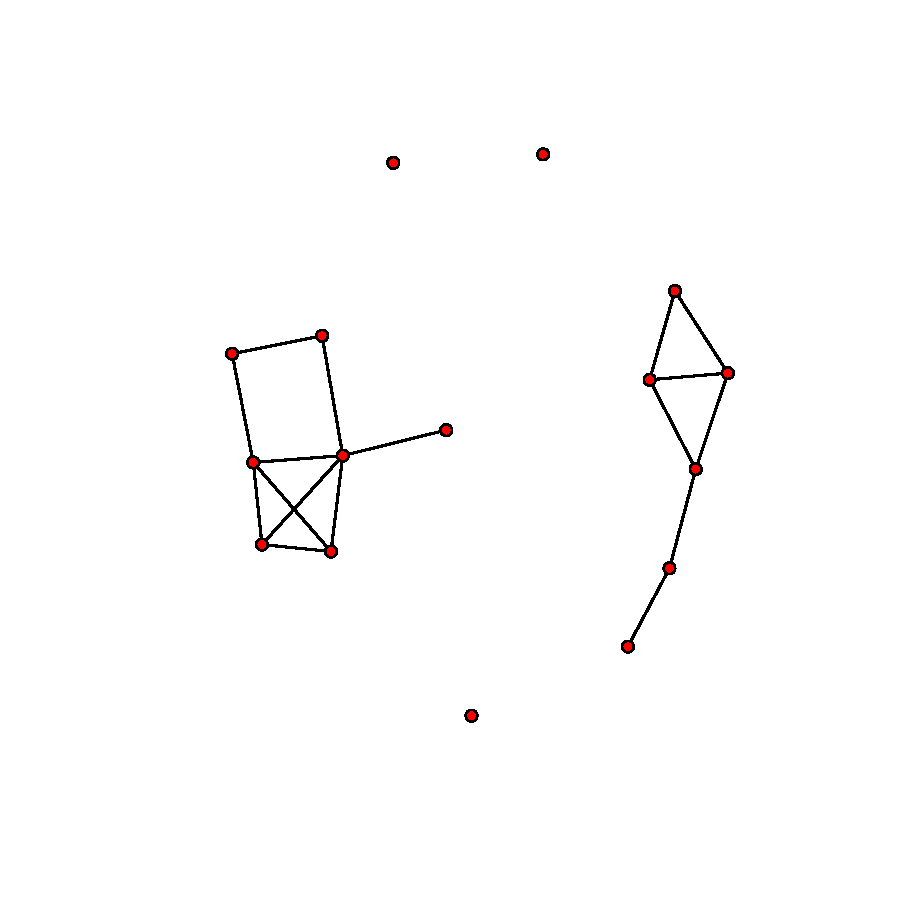
\includegraphics[height=3in]{STERGM-simex}
\end{center}
\end{figure}


How well do the cross-sectional networks within our simulated dynamic network fit the probability distribution implied by our model?  
We can check by considering the summary statistics for our observed network, and those for our cross-sectional networks.

\begin{Schunk}
\begin{Sinput}
> summary(flobusiness~edges+gwesp(0,fixed=T))
\end{Sinput}
\begin{Soutput}
        edges gwesp.fixed.0 
           15            12 
\end{Soutput}
\begin{Sinput}
> colMeans(attributes(flo.stergm.sim)$stats)
\end{Sinput}
\begin{Soutput}
        edges gwesp.fixed.0 
       18.134        14.756 
\end{Soutput}
\end{Schunk}

And we can also easily look at a time series and histogram for each statistic:

\begin{Schunk}
\begin{Sinput}
> plot(attributes(flo.stergm.sim)$stats)
\end{Sinput}
\end{Schunk}

\begin{figure}[ht]
\begin{center}
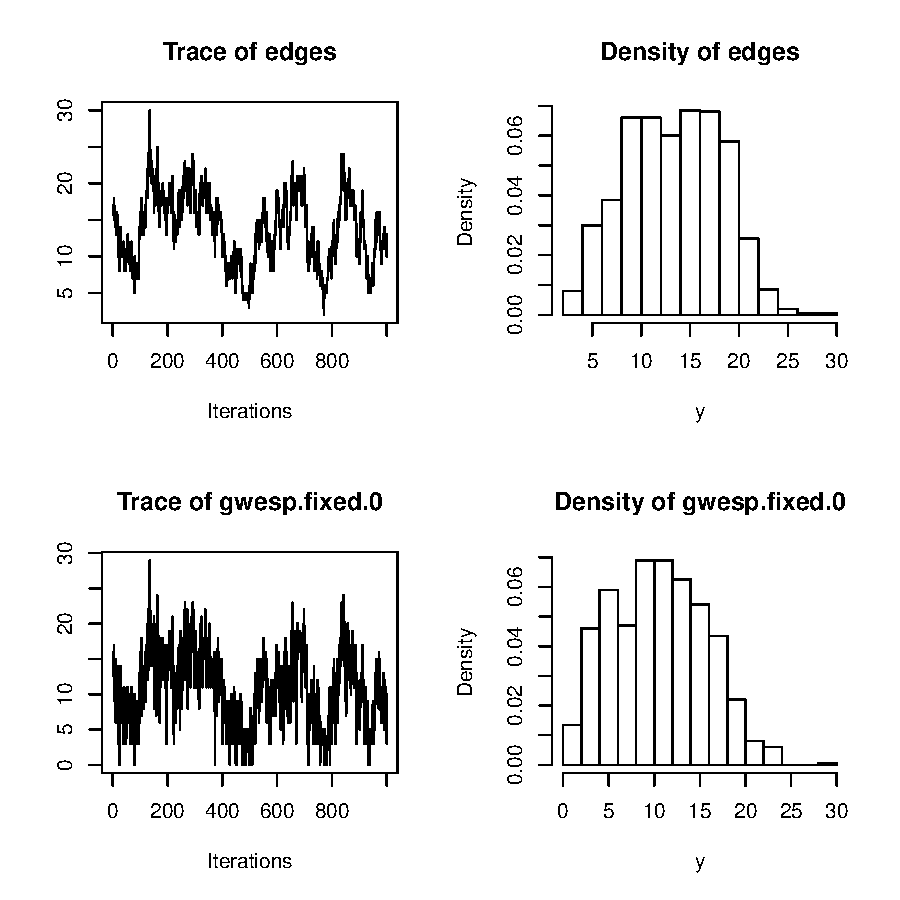
\includegraphics[height=3in]{STERGM-statsform1}
\end{center}
\end{figure}

We should also check to make sure that our mean duration is what we expect (10 time steps). This requires knowing an additional function: \texttt{as.data.frame}, 
which, when applied to an object of class \texttt{networkDynamic}, generates a timed edgelist. 
Although right-censoring is present for some edges in our simulation, with a mean duration of 10 time steps and a simulation 1000 time steps long, 
its effect on our observed mean duration should be trivial.

\begin{Schunk}
\begin{Sinput}
> flo.stergm.sim.dm <- as.data.frame(flo.stergm.sim)
> names(flo.stergm.sim.dm)
\end{Sinput}
\begin{Soutput}
[1] "start"          "end"            "tail"          
[4] "head"           "left.censored"  "right.censored"
[7] "duration"      
\end{Soutput}
\begin{Sinput}
> mean(flo.stergm.sim.dm$duration)
\end{Sinput}
\begin{Soutput}
[1] 9.999449
\end{Soutput}
\end{Schunk}

The information on when an edge is active and when it is inactive is stored within our \texttt{network} object as the edge attribute \texttt{active}.  
Vertices, too, are capable of becoming active and inactive within \texttt{networkDynamic}, and this information is stored as a vertex attribute.
Most of the time, users should access this information indirectly, through functions like \texttt{network.extract} or \texttt{as.data.frame}.  
Additional functions to query or set activity include \texttt{is.active}, \texttt{activate.vertex}, \texttt{deactivate.vertex}, \texttt{activate.edge},
and \texttt{deactivate.edge}, all documented in \texttt{help(package="networkDynamic")}.

For those who want to look under the hood, they can see the activity spells directly.  For a single edge, say, edge number 25, use:

\begin{Schunk}
\begin{Sinput}
> get.edge.value(flo.stergm.sim, "active", unlist=FALSE)[[25]]
\end{Sinput}
\begin{Soutput}
      [,1] [,2]
 [1,] -Inf   11
 [2,]   12   33
 [3,]  326  336
 [4,]  341  343
 [5,]  432  436
 [6,]  458  464
 [7,]  489  492
 [8,]  727  736
 [9,]  737  742
[10,]  743  755
[11,]  913  915
\end{Soutput}
\end{Schunk}

Note that \texttt{networkDynamic} stores spells in the form [onset,terminus), meaning that the spell is inclusive of the onset and exclusive of the terminus.  
So a spell of 3,7 means the edge begins at time point 3 and ends just before time point 7.  networkDynamic can handle continuous-time spell information.  
However, since STERGMs are discrete-time with integer steps, what this means for STERGM is that the edge is inactive up through time step 2;
 active at time steps 3, 4, 5, and 6; and inactive again at time step 7 and on. Its duration is thus 4 time steps.

\section{Example 3: Long durations and the Carnegie approximation}

Let us reconsider Example 2, with a mean relational duration of 100 time steps.

\begin{Schunk}
\begin{Sinput}
> theta.diss.100 <- log(99)
\end{Sinput}
\end{Schunk}

First, we treat the formation process as if it were a stand-alone cross-sectional model, and estimate it using a standard cross-sectional ERGM. 
We did, in fact, fit this cross-sectional model earlier:

\begin{Schunk}
\begin{Sinput}
> flo.stergm.approx <- ergm(flobusiness~edges+gwesp(0,fixed=T))
\end{Sinput}
\begin{Soutput}
Iteration 1 of at most 20: 
Convergence test P-value: 9.9e-259 
The log-likelihood improved by 0.07519 
Iteration 2 of at most 20: 
Convergence test P-value: 1.4e-41 
The log-likelihood improved by 0.01319 
Iteration 3 of at most 20: 
Convergence test P-value: 2.2e-08 
The log-likelihood improved by 0.003 
Iteration 4 of at most 20: 
Convergence test P-value: 3.3e-03 
The log-likelihood improved by 0.001035 
Iteration 5 of at most 20: 
Convergence test P-value: 1.9e-01 
The log-likelihood improved by 0.0003084 
Iteration 6 of at most 20: 
Convergence test P-value: 4.8e-01 
The log-likelihood improved by 0.0001593 
Iteration 7 of at most 20: 
Convergence test P-value: 5.9e-01 
Convergence detected. Stopping.
The log-likelihood improved by < 0.0001 

This model was fit using MCMC.  To examine model diagnostics and check for degeneracy, use the mcmc.diagnostics() function.
\end{Soutput}
\begin{Sinput}
> summary(flo.stergm.approx)
\end{Sinput}
\begin{Soutput}
==========================
Summary of model fit
==========================

Formula:   flobusiness ~ edges + gwesp(0, fixed = T)

Iterations:  20 

Monte Carlo MLE Results:
              Estimate Std. Error MCMC % p-value    
edges          -3.3674     0.6058      0 < 1e-04 ***
gwesp.fixed.0   1.5703     0.5752      0 0.00731 ** 
---
Signif. codes:  0 �***� 0.001 �**� 0.01 �*� 0.05 �.� 0.1 � � 1 

     Null Deviance:   0.00  on 120  degrees of freedom
 Residual Deviance: -88.07  on 118  degrees of freedom
 
AIC: -84.07    BIC: -78.49    (Smaller is better.) 
\end{Soutput}
\begin{Sinput}
> theta.form <- flo.stergm.approx$coef 
> theta.form
\end{Sinput}
\begin{Soutput}
        edges gwesp.fixed.0 
    -3.367363      1.570276 
\end{Soutput}
\end{Schunk}

Then, we subtract the values of the dissolution $\theta$ from each of the corresponding values in the formation model. 
In this example, the dissolution model contains only an edges term, so this coefficient should be subtracted from the starting value for the edges term in the formation model. 

\begin{Schunk}
\begin{Sinput}
> theta.form[1] <- theta.form[1] - theta.diss.100
\end{Sinput}
\end{Schunk}

How well does this approximation do in capturing our desired dynamic network properties? First, we can simulate from it:

\begin{Schunk}
\begin{Sinput}
> flo.stergm.sim.2 <- simulate(flobusiness,
 	formation=~edges+gwesp(0,fixed=T),
 	dissolution=~edges,
 	monitor="all",
 	coef.form=theta.form,
 	coef.diss=theta.diss.100,
 	time.slices=10000)
\end{Sinput}
\end{Schunk}

Then check the results in terms of cross-sectional network structure and mean relational duration?

\begin{Schunk}
\begin{Sinput}
> summary(flobusiness~edges+gwesp(0,fixed=T))
\end{Sinput}
\begin{Soutput}
        edges gwesp.fixed.0 
           15            12 
\end{Soutput}
\begin{Sinput}
> colMeans(attributes(flo.stergm.sim.2)$stats)
\end{Sinput}
\begin{Soutput}
        edges gwesp.fixed.0 
      13.7348       10.9880 
\end{Soutput}
\begin{Sinput}
> stergm.sim.dm.2 <- as.data.frame(flo.stergm.sim.2)
> mean(stergm.sim.dm.2$duration)
\end{Sinput}
\begin{Soutput}
[1] 98.03426
\end{Soutput}
\begin{Sinput}
> plot(attributes(flo.stergm.sim.2)$stats)
\end{Sinput}
\end{Schunk}

\begin{figure}[ht]
\begin{center}
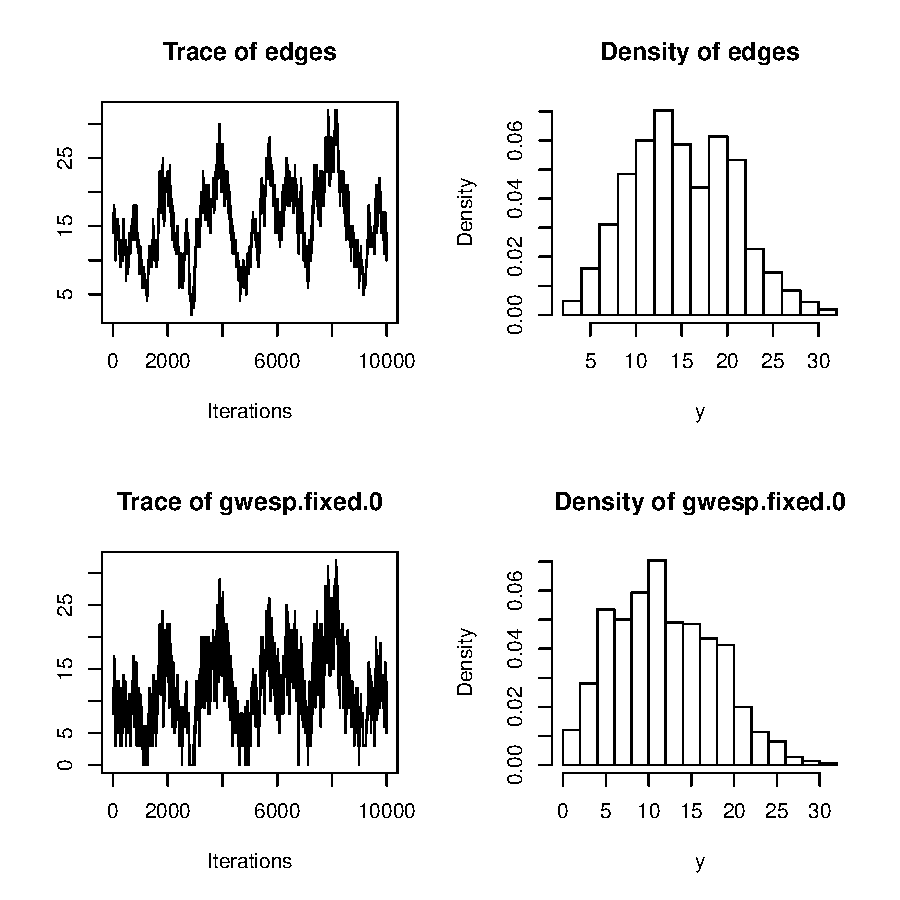
\includegraphics[height=3in]{STERGM-simform}
\end{center}
\end{figure}

\section{Example 4: Estimation and simulation driven by egocentric data}

Just like we saw with ergms, stergms can be modeled using only target statistics.  
For example, imagine that you want to model HIV transmission among a population of gay men in steady partnerships. 
50\% of the men are White and 50\% are Black. 
You collect egocentric partnership data from a random (ha! ha!) sample of these men. Your data say:

\begin{enumerate}
\item{There are no significant differences in the distribution of momentary degree (the number of ongoing partnerships at one point in time) 
reported by White vs. Black men. The mean is 0.90, and the overall distribution is:}
\begin{enumerate}
\item{36\% degree 0}
\item{46\% degree 1}
\item{18\% degree 2+}
\end{enumerate}
\item{83.3\% of relationships are racially homogeneous}
\end{enumerate}

We also have data (from these same men, or elsewhere) that tell us that the mean duration for a racially homogenous relationship is 10 months, 
while for a racially mixed one it is 20 months.  
(Perhaps this is because the social pressure against cross-race ties makes it such that those who are willing to enter them are a select group, 
more committed to their relationships).

Before we model the disease transmission, we need a dynamic network that possesses each of thse features to simulate it on. 

Our first step is to create a 500-node undirected network, and assign the first 250 nodes to race 0 and the second to race 1. The choice of 500 nodes is arbitary.

\begin{Schunk}
\begin{Sinput}
> msm.net <- network.initialize(500, directed=F)	
> msm.net %v% 'race' <- c(rep(0,250),rep(1,250))
> msm.net
\end{Sinput}
\begin{Soutput}
 Network attributes:
  vertices = 500 
  directed = FALSE 
  hyper = FALSE 
  loops = FALSE 
  multiple = FALSE 
  bipartite = FALSE 
  total edges= 0 
    missing edges= 0 
    non-missing edges= 0 

 Vertex attribute names: 
    race vertex.names 
\end{Soutput}
\end{Schunk}

ERGM and STERGM have functionality that allow us to simply state what the target statistics are that we want to match; we do not actually need to generate 
a network that has them.  The formation formula and target statistics that we need are:

\begin{Schunk}
\begin{Sinput}
> msm.form.formula <- ~edges+nodematch('race')+degree(0)+
     concurrent
> msm.target.stats <- c(225,187,180,90)
\end{Sinput}
\end{Schunk}

Why don't we specify \texttt{degree(1)} as well?
How did we get those values?

Now let us turn to dissolution. We are back to the case where we can solve these explicitly, 
although this is complicated slightly by the fact that our disslution probabilities differ by the race composition of the members.  
One dissolution formula for representing this is:

\begin{Schunk}
\begin{Sinput}
> msm.diss.formula <- ~offset(edges)+offset(nodematch("race"))
\end{Sinput}
\end{Schunk}

These two model statistics means that there will be two model coefficients.  Let us call them $\theta_1$ and $\theta_2$ for the edges and nodematch terms, respectively. 
Let us also refer to the change statistics for actor pair $i,j$ for each of these as $\delta_1(y_{ij})$ and $\delta_2(y_{ij})$, respectively.

Thus the log-odds expression for dissolution that we saw earlier would here be expressed as:
\begin{equation}\label{disslogit}
\ln{\frac{P(Y_{ij,t+1}=1 \mid Y_{ij,t}=1)}{P(Y_{ij,t+1}=0\mid Y_{ij,t}=1)}} = \theta_1\delta_1(y_{ij})+\theta_2\delta_2(y_{ij})
\end{equation}
Note that $\delta_1(y_{ij})$ would equal 1 for all actor pairs, while $\delta_2(y_{ij})$ would equal 1 for race homophilous pairs and 0 for others.  
That means that the log-odds of tie persistence will equal $\theta_1$ for mixed-race couples and $\theta_1 + \theta_2$ for race-homophilous couples.  
This suggests that we should be able to calculate $\theta_1$ directly, and subsequently calculate $\theta_2$.

Following the logic we saw in the Example 1, we can see that:
\begin{equation}
\theta_1 = \ln{d_{mixed}-1}
\end{equation}
and therefore $\theta_1 = \ln{(20-1)} = \ln{19} = 2.944$.

Furthermore, 
\begin{equation}
\theta_1 + \theta_2 = \ln{d_{homoph}-1}
\end{equation}
and therefore $\theta_2 = \ln{(d_{homoph}-1)}-\theta_1 = \ln{(10-1)} - 2.944 = -0.747$.

So, we have:

\begin{Schunk}
\begin{Sinput}
> msm.theta.diss <- c(2.944, -0.747) 
\end{Sinput}
\end{Schunk}

Putting it all together gives us:

\begin{Schunk}
\begin{Sinput}
> set.seed(0)
> msm.fit <- stergm(msm.net,
 	formation= msm.form.formula,
 	dissolution= msm.diss.formula,
 	targets="formation",
 	target.stats= msm.target.stats,
 	offset.coef.diss = msm.theta.diss,
 	estimate = "EGMME",
 	control=control.stergm(SA.plot.progress=TRUE)
 #		SA.phase2.levels.max=1)
 )
\end{Sinput}
\end{Schunk}

\texttt{Iteration 1 of at most 20:}\\
$\Rightarrow$ Lots of output snipped. $\Leftarrow$ \\
\texttt{========  Phase 3: Simulate from the fit and estimate standard errors. ========}\\

Let's first check to make sure it fit well:

\begin{Schunk}
\begin{Sinput}
> mcmc.diagnostics(msm.fit)
\end{Sinput}
\end{Schunk}
$\Rightarrow$ Lots of output snipped. $\Leftarrow$\\
\begin{figure}[h]
\begin{center}
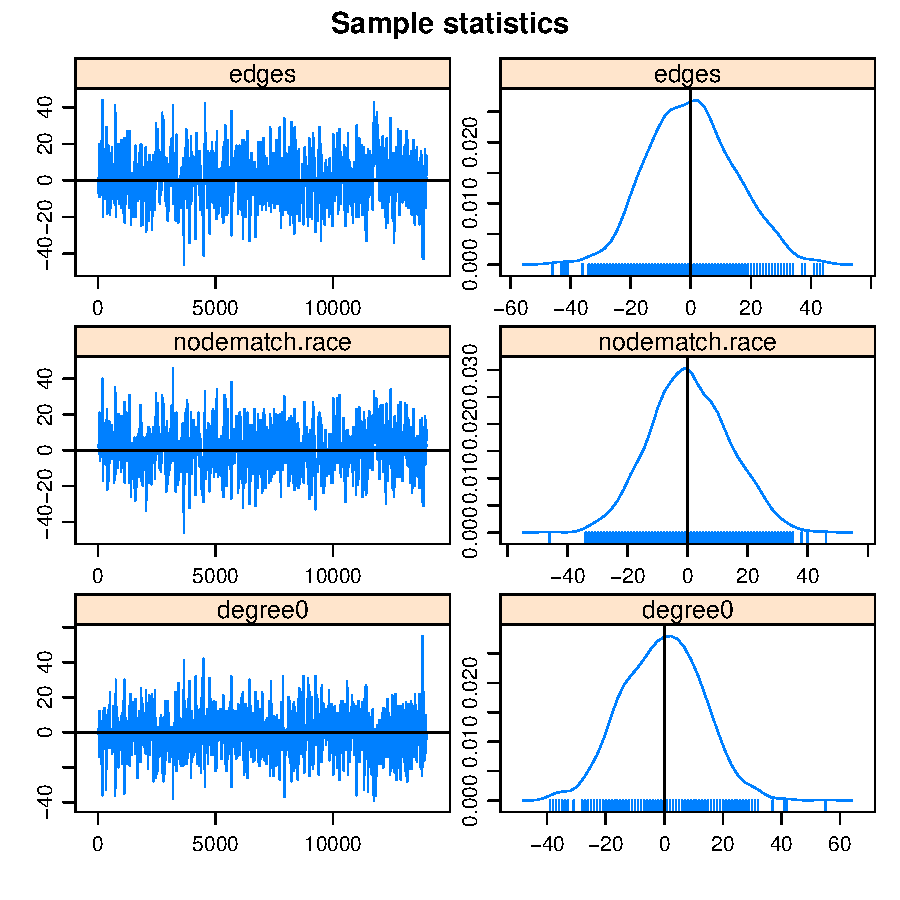
\includegraphics[height=3in]{STERGM-msmdiag}
\end{center}
\end{figure}

and see what the results tell us:

\begin{Schunk}
\begin{Sinput}
> summary(msm.fit)
\end{Sinput}
\begin{Soutput}
==============================
Summary of formation model fit 
==============================

Formula:   ~edges + nodematch("race") + degree(0) + concurrent

Iterations:  NA 

Equilibrium Generalized Method of Moments Results:
               Estimate Std. Error MCMC %  p-value    
edges           -9.9659     0.2241     NA  < 1e-04 ***
nodematch.race   2.3013     0.2208     NA  < 1e-04 ***
degree0         -0.2068     0.1194     NA 0.083200 .  
concurrent      -0.8263     0.2357     NA 0.000455 ***
---
Signif. codes:  0 �***� 0.001 �**� 0.01 �*� 0.05 �.� 0.1 � � 1 

Warning:  The standard errors do not incorporate uncertainty due to the "noisy" estimation procedure.


================================
Summary of dissolution model fit
================================

Formula:   ~offset(edges) + offset(nodematch("race"))

Iterations:  NA 

Equilibrium Generalized Method of Moments Results:
               Estimate Std. Error MCMC % p-value
edges             2.944         NA     NA      NA
nodematch.race   -0.747         NA     NA      NA

Warning:  The standard errors do not incorporate uncertainty due to the "noisy" estimation procedure.


 The following terms are fixed by offset and are not estimated:
  edges nodematch.race 
\end{Soutput}
\end{Schunk}

Now, we simulate a dynamic network:

\begin{Schunk}
\begin{Sinput}
> msm.sim <- simulate(msm.fit,time.slices=1000)
\end{Sinput}
\end{Schunk}

and compare the outputs to what we expect, in terms of cross-sectional structure:

\begin{Schunk}
\begin{Sinput}
> colMeans(attributes(msm.sim)$stats)
\end{Sinput}
\begin{Soutput}
         edges nodematch.race        degree0     concurrent 
       224.766        187.786        178.786         89.063 
\end{Soutput}
\begin{Sinput}
> msm.target.stats
\end{Sinput}
\begin{Soutput}
[1] 225 187 180  90
\end{Soutput}
\end{Schunk}

Here's another interesting way to look at one aspect of the network structure:

\begin{Schunk}
\begin{Sinput}
> msm.sim.dm <- as.data.frame(msm.sim)
> plot(msm.sim.dm$head,msm.sim.dm$tail)
\end{Sinput}
\end{Schunk}

\begin{figure}[ht]
\begin{center}
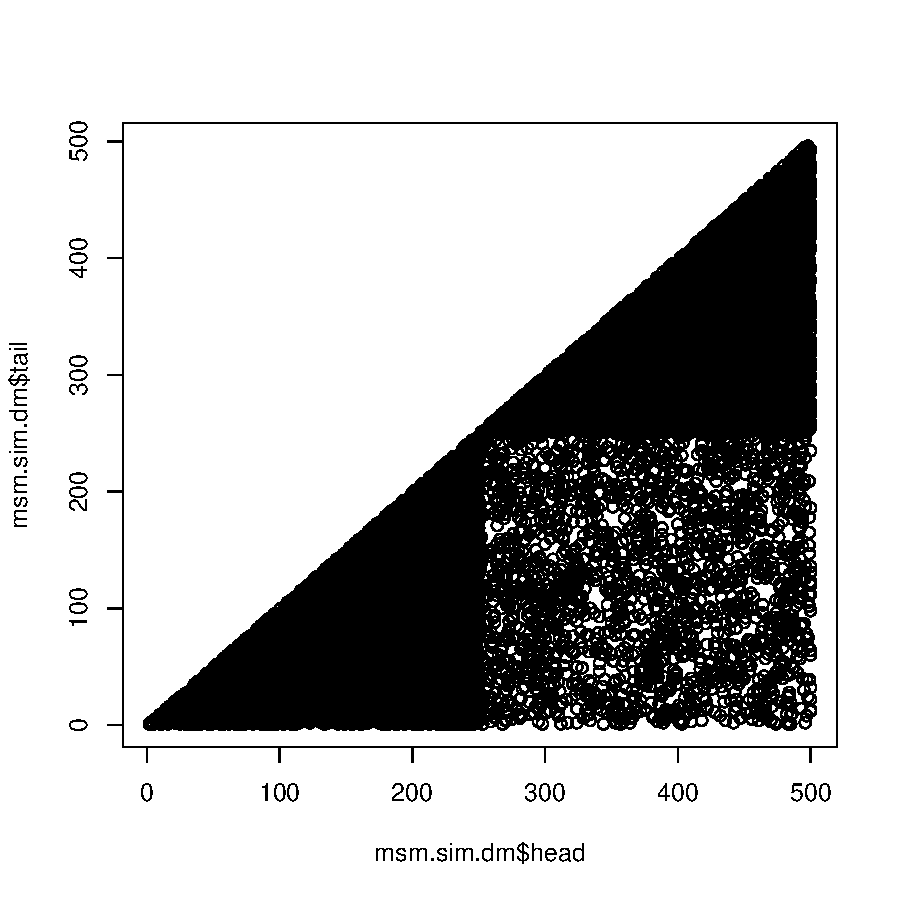
\includegraphics[height=3in]{STERGM-msmht}
\end{center}
\end{figure}
 
And relationship length:

\begin{Schunk}
\begin{Sinput}
> names(msm.sim.dm)
\end{Sinput}
\begin{Soutput}
[1] "start"          "end"            "tail"          
[4] "head"           "left.censored"  "right.censored"
[7] "duration"      
\end{Soutput}
\begin{Sinput}
> msm.sim.dm$race1 <- msm.sim.dm$head>250
> msm.sim.dm$race2 <- msm.sim.dm$tail>250
> msm.sim.dm$homoph <- msm.sim.dm$race1 == msm.sim.dm$race2
> mean(msm.sim.dm$duration[msm.sim.dm$homoph==T & 
   msm.sim.dm$left.censored==F & msm.sim.dm$right.censored==F ])
\end{Sinput}
\begin{Soutput}
[1] 9.942613
\end{Soutput}
\begin{Sinput}
> mean(msm.sim.dm$duration[msm.sim.dm$homoph==F & 
   msm.sim.dm$left.censored==F & msm.sim.dm$right.censored==F ])
\end{Sinput}
\begin{Soutput}
[1] 19.25297
\end{Soutput}
\end{Schunk}


\end{document}
